\documentclass{ppig}
\usepackage{epsfig, graphicx} % support for image encoding and manipulation
\usepackage{ucs} % support for using UTF-8 as input encoding in LaTeX
\usepackage[utf8x]{inputenc} % required for UTF-8 support with ucs.sty
\usepackage{tabularx, multirow, booktabs} % support for high-quality tables
\usepackage{csquotes} % support for block quotes (using displayquote command)

% The titlebox defines how much vertical space is given for
% the authors' list. If you need extra space to show all the
% authors, uncomment the line below and increase the value. Please
% do not make the titlebox smaller than the original size of 5cm.
%\setlength\titlebox{5cm}

\title{An Examination of IDE Design for Programming as Problem-Solving}

% List the authors like you would in a table.
% The \And command creates another author's column. Use it after the
% details of one author to separate them from the following author horizontally.
% The \AND command creates a new "row" of authors and it should be used
% when the authors don't fit on the same line. You may have to increase
% the titlebox so that the author's don't overlap with the abstract.
\author{Nicholas Nelson \\
  Electrical Engineering \&\\ Computer Science \\
  Oregon State University \\
  nelsonni@oregonstate.edu \\
  \And
  Anita Sarma \\
  Electrical Engineering \&\\ Computer Science \\
  Oregon State University \\
  Anita.Sarma@oregonstate.edu \\
  \And
  André van der Hoek \\
  Department of Informatics \\
  University of California, Irvine \\
  andre@ics.uci.edu
}
  
\date{\today}

% Packages and macros for editorial purposes. Not required for submission.
\usepackage{color}
\definecolor{darkgreen}{rgb}{0.0, 0.5, 0.0}
\definecolor{ballblue}{rgb}{0.13, 0.67, 0.8}
\definecolor{aoblue}{rgb}{0.0, 0.0, 1.0}
\newcommand{\bold}[1]{\textit{\textbf{\color{aoblue}#1}}} % macro for boldifications
\newcommand{\todo}[1]{\textit{\textbf{\color{red}TODO: #1}}} % macro for TODO items
\newcommand{\discuss}[1]{\textit{\textbf{\color{darkgreen}#1}}} % macro for in-line discussions/questions
\newcommand{\nameUI}{\textit{<Insert Name>} UI} % macro placeholder for the name of the UI
\usepackage{enumitem}

\begin{document}
\maketitle
\thispagestyle{empty}

\begin{abstract}

Programming is inherently a problem-solving exercise: A programmer has to cultivate an understanding of the situation, externalize and contextualize thoughts \& ideas, develop strategies on how to proceed with the task, enact changes according to the most appropriate strategy, and retrospectively learn from each problem.
Therefore, programming is clearly more than just code input, testing, and maintenance.
Current IDEs, however, largely focus on the "writing code" parts of programming.
In this paper, we revisit which activities and actions constitute programming, and highlight six challenges to supporting these activities.
We then briefly describe a new paradigm of interacting with the IDE that we are working on to more directly support each of the six activities. 
\end{abstract}

\section{Programming as Problem-Solving}

Programming is more than dealing with language syntax and semantics: it is inherently an exercise in problem-solving that extends beyond the act of editing code in an Integrated Development Environment (IDE).
We are not the first to observe this.
For instance, programming has been characterized as an iterative process of refining mental representations of computational problems and solutions and expressing those representations as code~\cite{loksa2016programming}.

As an example, Leslie Lamport once opened a lecture with the statement, ``no one just starts writing code and hopes it happens to implement a web browser''~\cite{lamport2015lecture}.
He was advocating for design and specification prior to coding, but this statement also highlights the insight that programming requires thinking in a problem-solving manner at higher levels of abstraction than code.
Further evidence for the fact that programming is more than just coding is promoted by studies that have highlighted that programming requires gathering information from multiple sources~\cite{sillito2008asking}, includes creating mental models of program structures~\cite{von1995comprehension}, and involves exploring and evaluating many alternatives~\cite{hartmann2008design}.

% Much is known already about programming being a problem-solving activity beyond editing code in the editor provided by the IDE.
% During software development, for instance, programmers are known to create all sorts of auxiliary non-code artifacts~\cite{cherubini2007whiteboard}.
% As a second example, programmers are known to organize these artifacts into structures that are relevant to the particular task(s) they are currently focused upon~\cite{baltes2016empirical}.
% As a final example, programmers are known to not pursue a single solution, but to generally approach a task by exploring (either mentally or externalized) multiple alternative solutions~\cite{madeyski2017experimentation}.
% By applying prior work on problem-solving from a cognitive psychology perspective~\cite{mayer1992thinking}, we can classify these actions, respectively, into \textit{representing relevant information}, \textit{contextualizing information}, and \textit{generating alternatives}.
% These actions can then be generalized to represent the problem-solving activities of \textit{externalizing thoughts \& ideas} and \textit{developing strategies}.

\begin{table}[!htbp]
\caption{Activities and Actions of Programming as Problem-Solving}
\label{pps_matrix}
\centering
\begin{tabular}{|c|c|l|}
	\hline
	\multicolumn{2}{|c|}{\textbf{Activities}} & \multicolumn{1}{|c|}{\textbf{Actions}}\\\hline
	\multirow{5}{*}{A1} & \multirow{5}{*}{Understanding the situation} & Identifying goals \\
		& & Recalling prior knowledge \\
		& & Constructing models \\
		& & Interpreting code artifacts \\
		& & Filling knowledge gaps \\\hline
	\multirow{3}{*}{A2} & \multirow{3}{*}{Externalizing thoughts \& ideas} & Representing relevant information \\
		& & Contextualizing information \\
		& & Preserving contextual information \\\hline
	\multirow{4}{*}{A3} & \multirow{4}{*}{Developing strategies} & Generating alternatives \\
		& & Articulating and refining alternatives \\
		& & Understanding and assessing alternatives \\
		& & Recombining aspects of alternatives \\\hline
	\multirow{3}{*}{A4} & \multirow{3}{*}{Enacting change} & Translating strategies to actions \\
		& & Tracking progress \\
		& & Evaluating and assessing change \\\hline
	\multirow{5}{*}{A5} & \multirow{5}{*}{Collaborate} & Feedback solicitation \\
		& & Team work \\
		& & Group think \\
		& & Leverage group knowledge \\
		& & Synchronization \\\hline
	\multirow{2}{*}{A6} & \multirow{2}{*}{Retrospect} & Reflect on work \\
		& & Preserve work \\\hline
\end{tabular}
\end{table} % Programming as Problem-Solving Matrix

We have surveyed the literature from the perspective of programming as problem-solving, leading to Table~\ref{pps_matrix} which summarizes problem-solving activities that developers employ during programming sessions.
Problem-solving in programming partitions into six categories (\textit{Activities} column), with specific actions  that represent in more detail how the high-level activities manifest themselves (\textit{Actions} column).
Clearly, not every task involves all of these problem-solving actions, and there is no linearity to the order in which they are employed.
Sometimes these actions may not even be observable when an action is done in the programmer's head.
At the same time, literature has documented that these activities do occur and play an important role in how programmers arrive at a solution to the programming problem at hand.

\section{Challenges}

Within this context, it is surprising that current IDEs only support some of this entire spectrum of programming activities, primarily focusing on support for navigating and editing the codebase.
Numerous challenges arise in current IDEs supporting the full set of actions that comprise problem-solving in programming.
These challenges span the different categories of activities (see Table~\ref{pps_matrix}, \textit{Activities} A1-A6), and even those activities (A4: \textit{enacting change}) that have traditionally been supported by IDEs have gaps in support when examined as problem-solving activities.

Supporting programmers in problem-solving is a difficult problem when we recognize that we need to understand human aspects such as how people think when programming, what development processes are required, what skills are best suited for the current problem, what knowledge already exists in relation to that problem, and what support (or lack thereof) already exists from previous problem solving efforts.
Therefore, creating an IDE that is meant to support all the different aspects of programming, from the problem-solving perspective, requires a careful analysis of both the individual aspects and their combinations.
We believe that it is necessary to fundamentally rethink IDEs.

To guide such a rethinking, the following challenges characterize what kind of novel support is needed for programming as problem-solving:

\begin{enumerate}
	\item \textit{\textbf{How to support programmers in formulating problems and reflecting on solutions?}}
	Programmers do not just arrive at a solution.
	They need to first \textit{contextualize} the computational problem in terms of what they know and how they can progress towards a possible solution.
	After which, they may explore, articulate, and reflect on different alternatives they try-- these activities are interleaved, sometimes even happening at the same time (e.g., a developer may reflect on the solution while they articulate it), and typically encompass several quick iterations.
	Often there is no single correct solution, and the best solution requires mixing and matching elements from multiple alternative solutions.
    
    \item \textit{\textbf{How to support programmers in viewing the relevant context in a problem space?}}
    No program is an island and the solution contained within it must exist in the context of the rest of the codebase and its related artifacts.
    Programmers need to understand where a code snippet fits in a codebase, what it calls out to, and what calls into it~\cite{desouza2008empirical}, the desired behaviors of the code snippet (e.g., computational speed, usability, feature sets), organizational policies (e.g., licensing, process standards, code style), and historical development (e.g., has a solution previously been tried and rejected).
    Information that defines the context is not always directly available, and instead, must be cobbled from different types of artifacts that span the codebase, design/requirement artifacts, communications records (i.e. handwritten, emails, group fileserver), edit history for project artifacts, etc.
    A developer needs to know where these individual pieces of information reside and how to cherry-pick the items that actually pertain to the problem at hand.
    
 	\item \textit{\textbf{How to support the variety of information processing and workflow styles of programmers?}}
 	Programmers exhibit creativity in their problem-solving activities, and the diversity of approaches means that no two programmers are the same.
 	Male programmers prefer to use a \textit{heuristic} (or \textit{selective}) approach that involves striving for efficiency by following contextually salient cues, whereas female programmers process information \textit{comprehensively}, seeking a more complete understanding of the problem~\cite{grigoreanu2012end}.
 	Visuospatial reasoning serves as a ubiquitous basis for abstract knowledge and inference, and is a core component to rationalizing the world around us~\cite{tversky2005visuospatial}.
 	When problem-solving, programmers bring their visuospatial reasoning and information processing style to bare when evaluating and organizing artifacts, solutions, and ideas.
  
  \item \textit{\textbf{How to support programmer understanding of the contextual history that lead to a solution?}}
  Problem-solving in programming does not occur in a vacuum, and neither is it a one-off activity.
  Programmers rely upon past experiences with similar problems, knowledge gained from previous interactions with the same set of artifacts, and memories of prior mental models that allowed comprehension and problem-solving to succeed.
  When solving a programming problem, programmers need to orient around both their own and others' problem-solving spaces in order to transition from contemplating into actualizing (enacting) a solution.
  
  \item \textit{\textbf{How to enable collaboration between programmers when problem-solving not just code, but all related artifacts?}}
  Organizing oneself in relation to a problem creates a cognitive load~\cite{sweller1988cognitive}, and this load only increases when one adds collaborators.
  When information is spread across multiple information sources (e.g., code, sketches, written notes), programmers quickly exceed the $7\pm2$ capacity of their short-term memory~\cite{lisman1995storage}.
  Therefore, programmers must conceptualize artifacts and information into abstractions that allow for both the pursuit of a solution and sharing in order to enable multiple problem-solvers to operate cohesively.
  
  \item \textit{\textbf{How to enable the use of all of this information and context to support the act of coding?}}
  Solutions to programming problems must eventually be represented in code.
  Therefore, programmers must convert their conceptual solutions into actual lines of code.
  This process is non-linear (i.e., coding sessions start and stop), concurrent with all other problem-solving activities, and loosely organized (e.g., solutions are partially implemented, abandoned, and recovered).
  Therefore, programmers must cope with high-complexity coding sessions in the pursuit of simple, elegant software solutions.
\end{enumerate}

\section{Toward A New IDE}

\todo{Remove this paragraph and weave citations into the description of the IDE}\\
Previous work on alternative UI models for IDEs have focused on expanding the interface to allow more dynamic interactions for code comprehension and orientation.
Bragdon et al. proposed a user interface comprised of lightweight, editable fragments called bubbles, which form concurrently visible working sets in an interface called Code Bubbles~\cite{bragdon2010bubbles}.
DeLine et al. explored leveraging spatial memory to keep developers oriented by providing an infinite zoomable surface for software development, called Code Canvas~\cite{deline2010canvas}.
And combining efforts, the Code Bubbles team at Brown University and the Code Canvas team at Microsoft Research jointly created Debugger Canvas which provides collections of code bubbles on a two-dimensional pan-and-zoom interface~\cite{deline2012debugger}.
The interface models developed by these teams provide both theoretical and practical experience into alternative UI designs that help to break the mold of the ``bento-box'' model of IDEs.
Henley and Fleming similarly examined the tedious nature of navigating large information spaces and sought to reduce this burden for developers through a code editor UI that consists of a patch grid and a ribbon for navigating quickly through sets of code~\cite{henley2014patchworks}.
Da Silva et al. proposed a conflict avoidance approach to developer coordination problems which combines Emerging Design and side-by-side presentation in an architecture called Lighthouse~\cite{dasilva2006lighthouse}.
The Lighthouse user interface provides time-sensitive information about parallel changes introduced to a shared codebase in a novel approach to information awareness between developers in a team environment.
We seek to take these experiments a step further and examine whether combining the paradigm of programming as problem-solving and alternative UI design can further enable developers to use their innate problem-solving abilities.

To address these challenges, we have begun a research effort that attempts to rethink the IDE from the ground up using the problem-solving perspective as a paradigm shift for evaluating our design rationale.
We use Code Bubbles~\cite{bragdon2010bubbles} and Code Canvas~\cite{deline2010canvas} as key inspirations for interface designs that eschew window-based interfaces and explore spatial interfaces allowing users to project meaning onto the layout of their development environment.
Extending the zoomable canvas of Code Canvas and the code bubble windows of Code Bubbles, we explore these and other concepts from interface design to support the problem-solving activities that programmers encounter.

Modern IDEs are comprised of different information sources being presented in a variety of visual elements that must be organized and comprehended by users.
According to the Gestalt school of thought, our perception of the world is influenced by the way we group and segregate the visual stimuli presented to us~\cite{kimchi2003perceptual}.
Instead of perceiving individual and distinct objects in the world, we perceive objects that are logically connected to each other~\cite{kimchi2003perceptual}.
The strength of grouping objects is inversely proportional to the distance between the elements~\cite{bergman2009peirce}; therefore, the closer the elements are to each other the stronger our perception is that these belong to the same group.
To take advantage of the neuro-cognitive process of perceptual organization, we propose a cards-based interface which allows card to be placed and stacked according to the logical organization that a user requires to develop a solution.

Programming activities span editing code to sketching ideas on whiteboards, with each action serving different problem-solving aspects in pursuit of a solution.
In order to support this variety of actions, we propose that cards in our cards-based interface come in different types that support specific information sources and interactions while providing a common platform.
These card types can include code editors for working with code in specific programming languages, sketchpads for both drawing ideas and annotating text, webpages for referencing information sources on the Internet, todo lists for organizing tasks, timelines for managing projects, emails and chat transcripts for communications, etc.

\begin{figure}[h!]
	\caption{Cards-based User Interface of a Problem-Solving IDE}
	\label{mockup}
	% trim={<left> <lower> <right> <upper>}
	\fbox{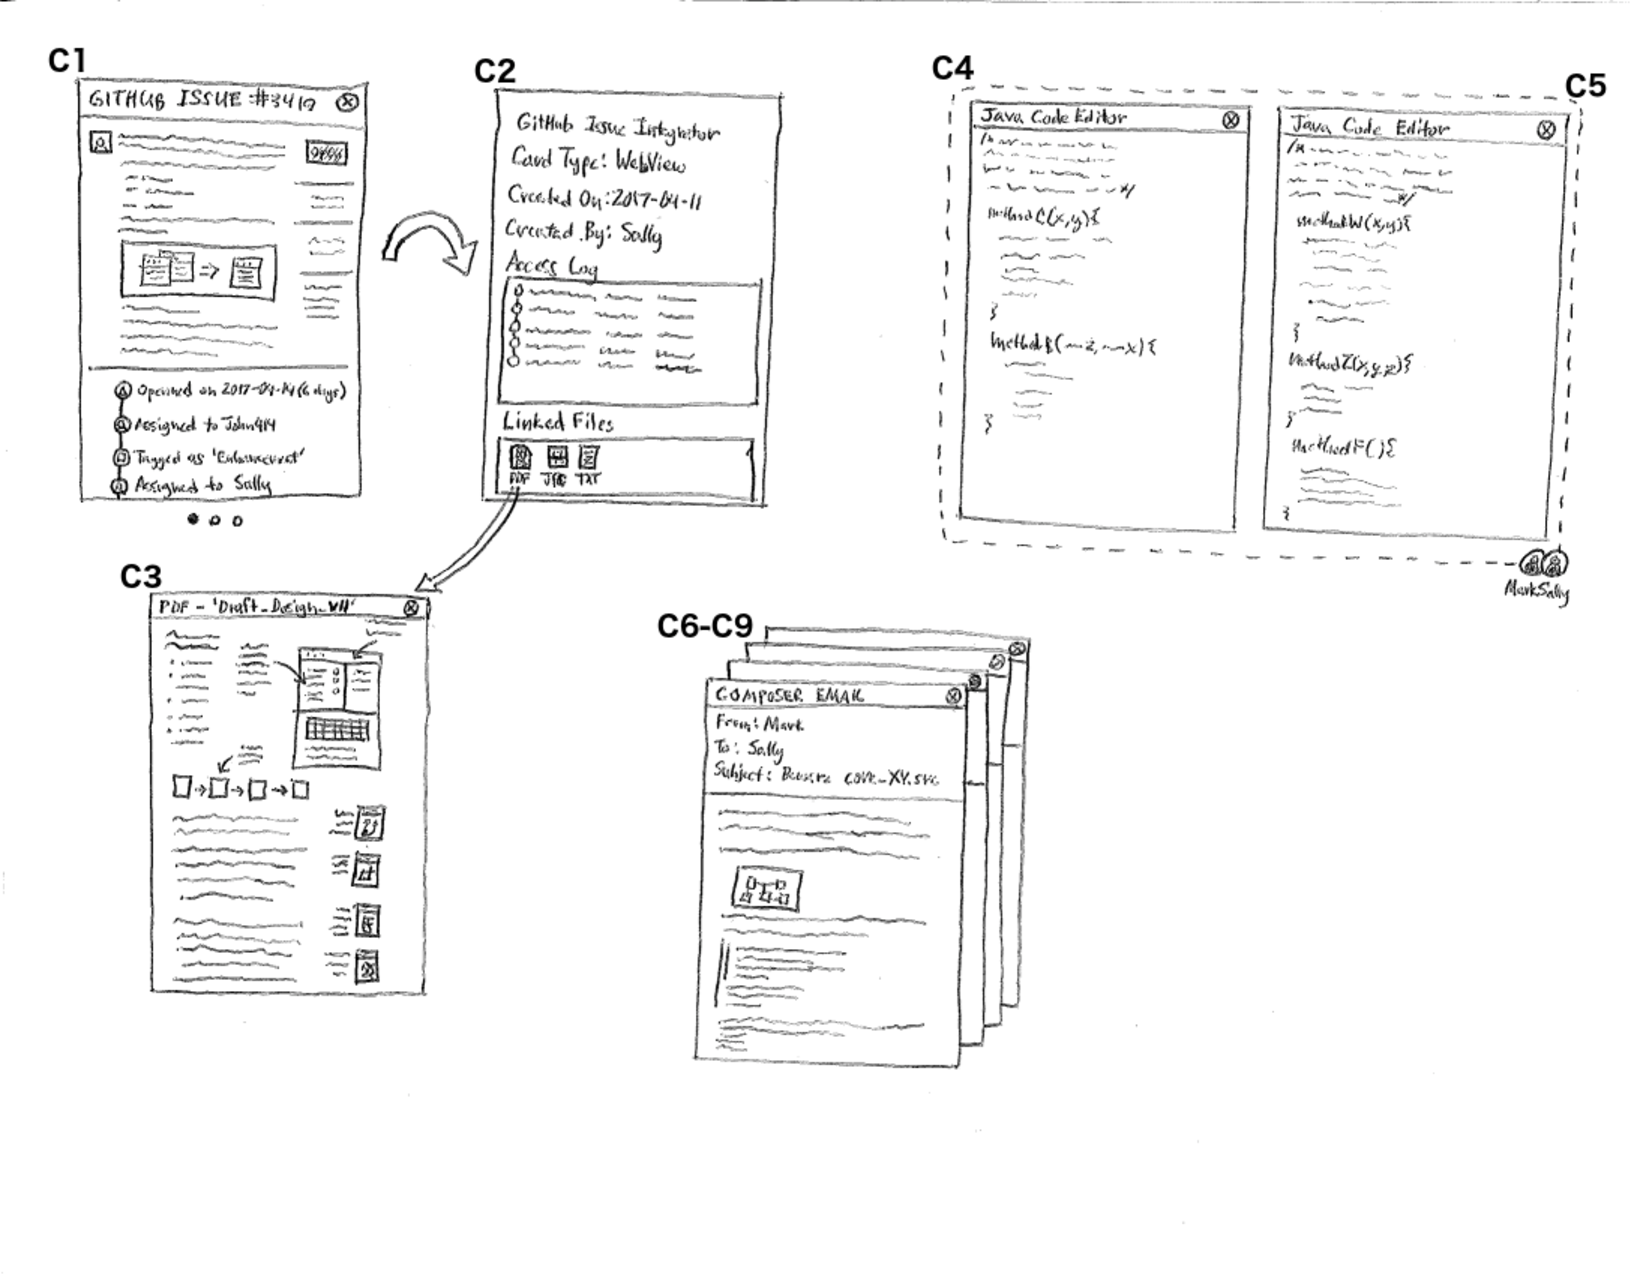
\includegraphics[trim={0.6cm 3.2cm 0.5cm 0.6cm},clip,width=\textwidth]{Mockup-9}}
	\vspace*{-1.5\baselineskip}
\end{figure}

\section{Applications}

To illustrate our proposed IDE, we present a high-fidelity interface design in Figure~\ref{mockup} and discuss the individual cards and stack elements contained within using a example scenario.
This scenario revolves around Sally, a junior developer tasked with updating the rendering engine within a web browser to use the latest API.
Her goal is a code-based solution to performing maintenance on a large and complex codebase, which requires prior design and forethought before enacting any changes.

Sally initially opens an issue tracker card (\texttt{C1}) that presents a condensed view of the description, tags, status, and history associated with her target issue.
The related issue on GitHub contains more activity events than can be presented on the card, and therefore an overflow indicator (three dots below the card) appears to give a visual cue that further information can be accessed via a swiping interaction.
Since Sally is interested in filling in her knowledge gaps about the issue, and any prior knowledge available, she flips the card around and examine the metadata on the back of the card.
The reverse card face (\texttt{C2}) contains meta-information related to when the card was originally opened, the card type, creator, access logs for the card, and any linked files.
Selecting the PDF \texttt{``Draft\_Design\_v11''}, Sally is able to launch a new PDF Viewer card (\texttt{C3}) that contains the sketches and notes from the design team.

Once Sally has grasped the available prior knowledge, contextualized it according to her task, and begun to develop strategies for completing the task she can open additional cards for code exploration and development.
Opening a Java Code Editor card (\texttt{C4}) that contains the target area of code that she will be modifying allows her to simultaneously reference documents from her previous information gathering while working on the code implementation.
Since Sally is not certain that her current changes will be the final solution, she can open an additional Java Code Editor card (\texttt{C5}) which contains the same target area of code prior to the introduction of her proposed changes (thus reflecting the checked-in version).
When reaching out to Mark, the senior developer on her team, Sally is able to select only the cards relevant to their conversation (\texttt{C4,C5}) and share them with Mark so that he can view them in his own IDE workspace.
These shared cards allow both Sally and Mark to edit code simultaneously and share thoughts and ideas without barriers that inhibit the exchange of shared knowledge.
If Mark, or any of the other stakeholders on the project, is unavailable for connecting to the shared cards and instead sends emails to Sally with ideas, sketches, and code snippets, Sally can open each of those emails in Composer Email cards (\texttt{C6-C9}) directly within her IDE workspace.
She can copy and paste the code snippets from the emails and into the Java Code Editor cards without having to switch between two separate applications and manage multiple associated windows.



This example illustrates the \textit{developing strategies} (A3) actions of \textit{generating alternatives}, \textit{articulating \& refining alternatives}, \textit{understanding \& assessing alternatives}, and \textit{recombining aspects of alternatives}.
Traditional IDEs have beenx incapable of supporting these types of activities without relying upon plugins or additional external applications.

\bibliography{bibliography}
\bibliographystyle{apacite} 
\end{document}
